\hypertarget{party_8h}{
\section{party.h File Reference}
\label{party_8h}\index{party.h@{party.h}}
}
{\tt \#include $<$R.h$>$}\par
{\tt \#include $<$Rmath.h$>$}\par
{\tt \#include $<$Rinternals.h$>$}\par
{\tt \#include $<$Rdefines.h$>$}\par
{\tt \#include $<$R\_\-ext/Applic.h$>$}\par
{\tt \#include $<$R\_\-ext/Lapack.h$>$}\par
{\tt \#include \char`\"{}Classes.h\char`\"{}}\par
{\tt \#include \char`\"{}Utils.h\char`\"{}}\par
{\tt \#include \char`\"{}mvt.h\char`\"{}}\par
{\tt \#include \char`\"{}LinearStatistic.h\char`\"{}}\par
{\tt \#include \char`\"{}TestStatistic.h\char`\"{}}\par
{\tt \#include \char`\"{}Distributions.h\char`\"{}}\par
{\tt \#include \char`\"{}Convenience.h\char`\"{}}\par
{\tt \#include \char`\"{}S3Classes.h\char`\"{}}\par
{\tt \#include \char`\"{}IndependenceTest.h\char`\"{}}\par
{\tt \#include \char`\"{}Splits.h\char`\"{}}\par
{\tt \#include \char`\"{}Node.h\char`\"{}}\par
{\tt \#include \char`\"{}Predict.h\char`\"{}}\par
{\tt \#include \char`\"{}SurrogateSplits.h\char`\"{}}\par
{\tt \#include \char`\"{}TreeGrow.h\char`\"{}}\par


Include dependency graph for party.h:\nopagebreak
\begin{figure}[H]
\begin{center}
\leavevmode
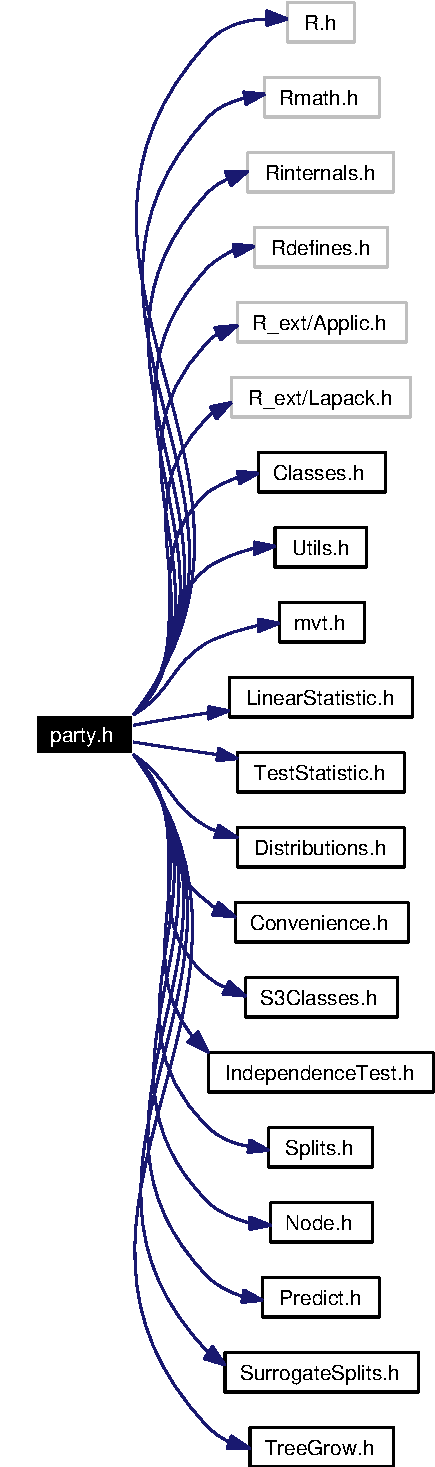
\includegraphics[width=420pt]{party_8h__incl}
\end{center}
\end{figure}


This graph shows which files directly or indirectly include this file:\nopagebreak
\begin{figure}[H]
\begin{center}
\leavevmode
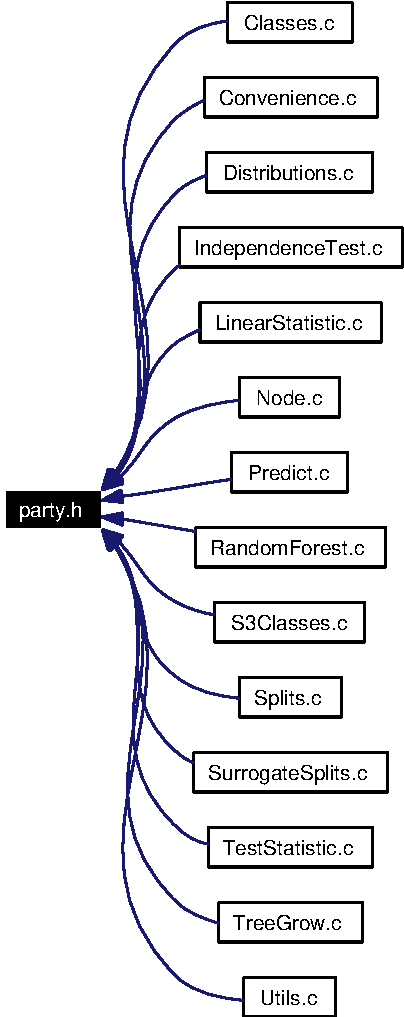
\includegraphics[width=420pt]{party_8h__dep__incl}
\end{center}
\end{figure}
\subsection*{Defines}
\begin{CompactItemize}
\item 
\#define \hyperlink{party_8h_2da0c160b5b1b6ae134b58720c204e32}{S3\_\-NODEID}~0
\item 
\#define \hyperlink{party_8h_1b80a31c6121bcb2218dce0034ee32a3}{S3\_\-WEIGHTS}~1
\item 
\#define \hyperlink{party_8h_1bb10765b7c7e74f8dbf7fbf0ab8b354}{S3\_\-CRITERION}~2
\item 
\#define \hyperlink{party_8h_0cebf7765e9de94702c0d4a8d35349b2}{S3\_\-TERMINAL}~3
\item 
\#define \hyperlink{party_8h_1508d011dbd56d47c17c718594128e88}{S3\_\-PSPLIT}~4
\item 
\#define \hyperlink{party_8h_6cbdd6966d49343e19eff3f80bc05303}{S3\_\-SSPLIT}~5
\item 
\#define \hyperlink{party_8h_dab41315603030e3d85038f40225e8e8}{S3\_\-PREDICTION}~6
\item 
\#define \hyperlink{party_8h_e6b64412ed72a9b5f4af50dbdeb46f5f}{S3\_\-LEFT}~7
\item 
\#define \hyperlink{party_8h_e884fc8af7f5510edd5102e07bf1bf7c}{S3\_\-RIGHT}~8
\item 
\#define \hyperlink{party_8h_03408349cc8dbd04a36733dfebffbacf}{S3\_\-SUMWEIGHTS}~9
\item 
\#define \hyperlink{party_8h_2594b3a85c654c34048133cb81ad0fab}{NODE\_\-LENGTH}~10
\item 
\#define \hyperlink{party_8h_7d9196a92b820e0fc23e59cdc69ae6c2}{S3\_\-STATISTICS}~0
\item 
\#define \hyperlink{party_8h_52cb7f77de1df6dd9b93078908c52816}{S3\_\-iCRITERION}~1
\item 
\#define \hyperlink{party_8h_70a64de1fafbdb4e40d57b867589ff97}{S3\_\-MAXCRITERION}~2
\item 
\#define \hyperlink{party_8h_9f26fcd39efae230d792a03c810c87a8}{CRITERION\_\-LENGTH}~3
\item 
\#define \hyperlink{party_8h_fe45cf6305b9f8e720fcbcfea32e8a79}{S3\_\-VARIABLEID}~0
\item 
\#define \hyperlink{party_8h_b98a5267036c4722529cbf1d28405d5c}{S3\_\-ORDERED}~1
\item 
\#define \hyperlink{party_8h_de7a9f1e1a374e0afa0e2b7d813cc0e7}{S3\_\-SPLITPOINT}~2
\item 
\#define \hyperlink{party_8h_727d68d7c6c0d885ff374a8779ebaab3}{S3\_\-SPLITSTATISTICS}~3
\item 
\#define \hyperlink{party_8h_e11d1d0e0fea5c655d40bd14dbf67e29}{S3\_\-TOLEFT}~4
\item 
\#define \hyperlink{party_8h_ea4e21f37dd3fddc02ad6d030e7f0e8f}{S3\_\-TABLE}~5
\item 
\#define \hyperlink{party_8h_27e42cfa9f63fb89059ef54f981d76fa}{SPLIT\_\-LENGTH}~6
\item 
\#define \hyperlink{party_8h_519bce0ae6bcf7c9ea49e687104a7e89}{MAXABS}~1
\item 
\#define \hyperlink{party_8h_2bb5fe1fde38878e1bc17e63950e3267}{QUADFORM}~2
\item 
\#define \hyperlink{party_8h_e58f101919f3367c51322fc2995f8286}{BONFERRONI}~1
\item 
\#define \hyperlink{party_8h_fe09ae6cccfcacdf668872522cf79528}{MONTECARLO}~2
\item 
\#define \hyperlink{party_8h_4df9c9469e4a30c16e8b9cdb2c95fd4f}{AGGREGATED}~3
\item 
\#define \hyperlink{party_8h_2fb8ad2edef6428fdcdbf04184164698}{UNIVARIATE}~4
\item 
\#define \hyperlink{party_8h_a37c25590457814f19baaa576ef3e54f}{TESTSTATISTIC}~5
\end{CompactItemize}


\subsection{Define Documentation}
\hypertarget{party_8h_4df9c9469e4a30c16e8b9cdb2c95fd4f}{
\index{party.h@{party.h}!AGGREGATED@{AGGREGATED}}
\index{AGGREGATED@{AGGREGATED}!party.h@{party.h}}
\subsubsection[{AGGREGATED}]{\setlength{\rightskip}{0pt plus 5cm}\#define AGGREGATED~3}}
\label{party_8h_4df9c9469e4a30c16e8b9cdb2c95fd4f}




Definition at line 68 of file party.h.

Referenced by C\_\-GlobalTest().\hypertarget{party_8h_e58f101919f3367c51322fc2995f8286}{
\index{party.h@{party.h}!BONFERRONI@{BONFERRONI}}
\index{BONFERRONI@{BONFERRONI}!party.h@{party.h}}
\subsubsection[{BONFERRONI}]{\setlength{\rightskip}{0pt plus 5cm}\#define BONFERRONI~1}}
\label{party_8h_e58f101919f3367c51322fc2995f8286}




Definition at line 66 of file party.h.

Referenced by C\_\-GlobalTest().\hypertarget{party_8h_9f26fcd39efae230d792a03c810c87a8}{
\index{party.h@{party.h}!CRITERION\_\-LENGTH@{CRITERION\_\-LENGTH}}
\index{CRITERION\_\-LENGTH@{CRITERION\_\-LENGTH}!party.h@{party.h}}
\subsubsection[{CRITERION\_\-LENGTH}]{\setlength{\rightskip}{0pt plus 5cm}\#define CRITERION\_\-LENGTH~3}}
\label{party_8h_9f26fcd39efae230d792a03c810c87a8}




Definition at line 50 of file party.h.

Referenced by C\_\-init\_\-node().\hypertarget{party_8h_519bce0ae6bcf7c9ea49e687104a7e89}{
\index{party.h@{party.h}!MAXABS@{MAXABS}}
\index{MAXABS@{MAXABS}!party.h@{party.h}}
\subsubsection[{MAXABS}]{\setlength{\rightskip}{0pt plus 5cm}\#define MAXABS~1}}
\label{party_8h_519bce0ae6bcf7c9ea49e687104a7e89}




Definition at line 62 of file party.h.

Referenced by C\_\-ConditionalPvalue().\hypertarget{party_8h_fe09ae6cccfcacdf668872522cf79528}{
\index{party.h@{party.h}!MONTECARLO@{MONTECARLO}}
\index{MONTECARLO@{MONTECARLO}!party.h@{party.h}}
\subsubsection[{MONTECARLO}]{\setlength{\rightskip}{0pt plus 5cm}\#define MONTECARLO~2}}
\label{party_8h_fe09ae6cccfcacdf668872522cf79528}




Definition at line 67 of file party.h.

Referenced by C\_\-GlobalTest().\hypertarget{party_8h_2594b3a85c654c34048133cb81ad0fab}{
\index{party.h@{party.h}!NODE\_\-LENGTH@{NODE\_\-LENGTH}}
\index{NODE\_\-LENGTH@{NODE\_\-LENGTH}!party.h@{party.h}}
\subsubsection[{NODE\_\-LENGTH}]{\setlength{\rightskip}{0pt plus 5cm}\#define NODE\_\-LENGTH~10}}
\label{party_8h_2594b3a85c654c34048133cb81ad0fab}




Definition at line 44 of file party.h.

Referenced by C\_\-init\_\-node(), C\_\-splitnode(), R\_\-Ensemble(), R\_\-Node(), and R\_\-TreeGrow().\hypertarget{party_8h_2bb5fe1fde38878e1bc17e63950e3267}{
\index{party.h@{party.h}!QUADFORM@{QUADFORM}}
\index{QUADFORM@{QUADFORM}!party.h@{party.h}}
\subsubsection[{QUADFORM}]{\setlength{\rightskip}{0pt plus 5cm}\#define QUADFORM~2}}
\label{party_8h_2bb5fe1fde38878e1bc17e63950e3267}




Definition at line 63 of file party.h.

Referenced by C\_\-ConditionalPvalue().\hypertarget{party_8h_1bb10765b7c7e74f8dbf7fbf0ab8b354}{
\index{party.h@{party.h}!S3\_\-CRITERION@{S3\_\-CRITERION}}
\index{S3\_\-CRITERION@{S3\_\-CRITERION}!party.h@{party.h}}
\subsubsection[{S3\_\-CRITERION}]{\setlength{\rightskip}{0pt plus 5cm}\#define S3\_\-CRITERION~2}}
\label{party_8h_1bb10765b7c7e74f8dbf7fbf0ab8b354}




Definition at line 36 of file party.h.

Referenced by C\_\-init\_\-node(), S3get\_\-criterion(), S3get\_\-maxcriterion(), and S3get\_\-teststat().\hypertarget{party_8h_52cb7f77de1df6dd9b93078908c52816}{
\index{party.h@{party.h}!S3\_\-iCRITERION@{S3\_\-iCRITERION}}
\index{S3\_\-iCRITERION@{S3\_\-iCRITERION}!party.h@{party.h}}
\subsubsection[{S3\_\-iCRITERION}]{\setlength{\rightskip}{0pt plus 5cm}\#define S3\_\-iCRITERION~1}}
\label{party_8h_52cb7f77de1df6dd9b93078908c52816}




Definition at line 48 of file party.h.

Referenced by C\_\-init\_\-node(), and S3get\_\-criterion().\hypertarget{party_8h_e6b64412ed72a9b5f4af50dbdeb46f5f}{
\index{party.h@{party.h}!S3\_\-LEFT@{S3\_\-LEFT}}
\index{S3\_\-LEFT@{S3\_\-LEFT}!party.h@{party.h}}
\subsubsection[{S3\_\-LEFT}]{\setlength{\rightskip}{0pt plus 5cm}\#define S3\_\-LEFT~7}}
\label{party_8h_e6b64412ed72a9b5f4af50dbdeb46f5f}




Definition at line 41 of file party.h.

Referenced by C\_\-splitnode(), C\_\-surrogates(), and S3get\_\-leftnode().\hypertarget{party_8h_70a64de1fafbdb4e40d57b867589ff97}{
\index{party.h@{party.h}!S3\_\-MAXCRITERION@{S3\_\-MAXCRITERION}}
\index{S3\_\-MAXCRITERION@{S3\_\-MAXCRITERION}!party.h@{party.h}}
\subsubsection[{S3\_\-MAXCRITERION}]{\setlength{\rightskip}{0pt plus 5cm}\#define S3\_\-MAXCRITERION~2}}
\label{party_8h_70a64de1fafbdb4e40d57b867589ff97}




Definition at line 49 of file party.h.

Referenced by C\_\-init\_\-node(), and S3get\_\-maxcriterion().\hypertarget{party_8h_2da0c160b5b1b6ae134b58720c204e32}{
\index{party.h@{party.h}!S3\_\-NODEID@{S3\_\-NODEID}}
\index{S3\_\-NODEID@{S3\_\-NODEID}!party.h@{party.h}}
\subsubsection[{S3\_\-NODEID}]{\setlength{\rightskip}{0pt plus 5cm}\#define S3\_\-NODEID~0}}
\label{party_8h_2da0c160b5b1b6ae134b58720c204e32}




Definition at line 34 of file party.h.

Referenced by C\_\-init\_\-node(), S3get\_\-nodeID(), and S3set\_\-nodeID().\hypertarget{party_8h_b98a5267036c4722529cbf1d28405d5c}{
\index{party.h@{party.h}!S3\_\-ORDERED@{S3\_\-ORDERED}}
\index{S3\_\-ORDERED@{S3\_\-ORDERED}!party.h@{party.h}}
\subsubsection[{S3\_\-ORDERED}]{\setlength{\rightskip}{0pt plus 5cm}\#define S3\_\-ORDERED~1}}
\label{party_8h_b98a5267036c4722529cbf1d28405d5c}




Definition at line 54 of file party.h.

Referenced by C\_\-init\_\-nominalsplit(), C\_\-init\_\-orderedsplit(), S3is\_\-ordered(), S3set\_\-nominal(), and S3set\_\-ordered().\hypertarget{party_8h_dab41315603030e3d85038f40225e8e8}{
\index{party.h@{party.h}!S3\_\-PREDICTION@{S3\_\-PREDICTION}}
\index{S3\_\-PREDICTION@{S3\_\-PREDICTION}!party.h@{party.h}}
\subsubsection[{S3\_\-PREDICTION}]{\setlength{\rightskip}{0pt plus 5cm}\#define S3\_\-PREDICTION~6}}
\label{party_8h_dab41315603030e3d85038f40225e8e8}




Definition at line 40 of file party.h.

Referenced by C\_\-init\_\-node(), and S3get\_\-prediction().\hypertarget{party_8h_1508d011dbd56d47c17c718594128e88}{
\index{party.h@{party.h}!S3\_\-PSPLIT@{S3\_\-PSPLIT}}
\index{S3\_\-PSPLIT@{S3\_\-PSPLIT}!party.h@{party.h}}
\subsubsection[{S3\_\-PSPLIT}]{\setlength{\rightskip}{0pt plus 5cm}\#define S3\_\-PSPLIT~4}}
\label{party_8h_1508d011dbd56d47c17c718594128e88}




Definition at line 38 of file party.h.

Referenced by C\_\-init\_\-node(), and S3get\_\-primarysplit().\hypertarget{party_8h_e884fc8af7f5510edd5102e07bf1bf7c}{
\index{party.h@{party.h}!S3\_\-RIGHT@{S3\_\-RIGHT}}
\index{S3\_\-RIGHT@{S3\_\-RIGHT}!party.h@{party.h}}
\subsubsection[{S3\_\-RIGHT}]{\setlength{\rightskip}{0pt plus 5cm}\#define S3\_\-RIGHT~8}}
\label{party_8h_e884fc8af7f5510edd5102e07bf1bf7c}




Definition at line 42 of file party.h.

Referenced by C\_\-splitnode(), and S3get\_\-rightnode().\hypertarget{party_8h_de7a9f1e1a374e0afa0e2b7d813cc0e7}{
\index{party.h@{party.h}!S3\_\-SPLITPOINT@{S3\_\-SPLITPOINT}}
\index{S3\_\-SPLITPOINT@{S3\_\-SPLITPOINT}!party.h@{party.h}}
\subsubsection[{S3\_\-SPLITPOINT}]{\setlength{\rightskip}{0pt plus 5cm}\#define S3\_\-SPLITPOINT~2}}
\label{party_8h_de7a9f1e1a374e0afa0e2b7d813cc0e7}




Definition at line 55 of file party.h.

Referenced by C\_\-init\_\-nominalsplit(), C\_\-init\_\-orderedsplit(), and S3get\_\-splitpoint().\hypertarget{party_8h_727d68d7c6c0d885ff374a8779ebaab3}{
\index{party.h@{party.h}!S3\_\-SPLITSTATISTICS@{S3\_\-SPLITSTATISTICS}}
\index{S3\_\-SPLITSTATISTICS@{S3\_\-SPLITSTATISTICS}!party.h@{party.h}}
\subsubsection[{S3\_\-SPLITSTATISTICS}]{\setlength{\rightskip}{0pt plus 5cm}\#define S3\_\-SPLITSTATISTICS~3}}
\label{party_8h_727d68d7c6c0d885ff374a8779ebaab3}




Definition at line 56 of file party.h.

Referenced by C\_\-init\_\-nominalsplit(), C\_\-init\_\-orderedsplit(), and S3get\_\-splitstatistics().\hypertarget{party_8h_6cbdd6966d49343e19eff3f80bc05303}{
\index{party.h@{party.h}!S3\_\-SSPLIT@{S3\_\-SSPLIT}}
\index{S3\_\-SSPLIT@{S3\_\-SSPLIT}!party.h@{party.h}}
\subsubsection[{S3\_\-SSPLIT}]{\setlength{\rightskip}{0pt plus 5cm}\#define S3\_\-SSPLIT~5}}
\label{party_8h_6cbdd6966d49343e19eff3f80bc05303}




Definition at line 39 of file party.h.

Referenced by C\_\-init\_\-node(), and S3get\_\-surrogatesplits().\hypertarget{party_8h_7d9196a92b820e0fc23e59cdc69ae6c2}{
\index{party.h@{party.h}!S3\_\-STATISTICS@{S3\_\-STATISTICS}}
\index{S3\_\-STATISTICS@{S3\_\-STATISTICS}!party.h@{party.h}}
\subsubsection[{S3\_\-STATISTICS}]{\setlength{\rightskip}{0pt plus 5cm}\#define S3\_\-STATISTICS~0}}
\label{party_8h_7d9196a92b820e0fc23e59cdc69ae6c2}




Definition at line 47 of file party.h.

Referenced by C\_\-init\_\-node(), and S3get\_\-teststat().\hypertarget{party_8h_03408349cc8dbd04a36733dfebffbacf}{
\index{party.h@{party.h}!S3\_\-SUMWEIGHTS@{S3\_\-SUMWEIGHTS}}
\index{S3\_\-SUMWEIGHTS@{S3\_\-SUMWEIGHTS}!party.h@{party.h}}
\subsubsection[{S3\_\-SUMWEIGHTS}]{\setlength{\rightskip}{0pt plus 5cm}\#define S3\_\-SUMWEIGHTS~9}}
\label{party_8h_03408349cc8dbd04a36733dfebffbacf}




Definition at line 43 of file party.h.

Referenced by C\_\-init\_\-node(), C\_\-Node(), and S3get\_\-sumweights().\hypertarget{party_8h_ea4e21f37dd3fddc02ad6d030e7f0e8f}{
\index{party.h@{party.h}!S3\_\-TABLE@{S3\_\-TABLE}}
\index{S3\_\-TABLE@{S3\_\-TABLE}!party.h@{party.h}}
\subsubsection[{S3\_\-TABLE}]{\setlength{\rightskip}{0pt plus 5cm}\#define S3\_\-TABLE~5}}
\label{party_8h_ea4e21f37dd3fddc02ad6d030e7f0e8f}




Definition at line 58 of file party.h.

Referenced by C\_\-init\_\-nominalsplit(), C\_\-init\_\-orderedsplit(), and S3get\_\-table().\hypertarget{party_8h_0cebf7765e9de94702c0d4a8d35349b2}{
\index{party.h@{party.h}!S3\_\-TERMINAL@{S3\_\-TERMINAL}}
\index{S3\_\-TERMINAL@{S3\_\-TERMINAL}!party.h@{party.h}}
\subsubsection[{S3\_\-TERMINAL}]{\setlength{\rightskip}{0pt plus 5cm}\#define S3\_\-TERMINAL~3}}
\label{party_8h_0cebf7765e9de94702c0d4a8d35349b2}




Definition at line 37 of file party.h.

Referenced by C\_\-init\_\-node(), S3get\_\-nodeterminal(), and S3set\_\-nodeterminal().\hypertarget{party_8h_e11d1d0e0fea5c655d40bd14dbf67e29}{
\index{party.h@{party.h}!S3\_\-TOLEFT@{S3\_\-TOLEFT}}
\index{S3\_\-TOLEFT@{S3\_\-TOLEFT}!party.h@{party.h}}
\subsubsection[{S3\_\-TOLEFT}]{\setlength{\rightskip}{0pt plus 5cm}\#define S3\_\-TOLEFT~4}}
\label{party_8h_e11d1d0e0fea5c655d40bd14dbf67e29}




Definition at line 57 of file party.h.

Referenced by C\_\-init\_\-nominalsplit(), C\_\-init\_\-orderedsplit(), S3get\_\-toleft(), and S3set\_\-toleft().\hypertarget{party_8h_fe45cf6305b9f8e720fcbcfea32e8a79}{
\index{party.h@{party.h}!S3\_\-VARIABLEID@{S3\_\-VARIABLEID}}
\index{S3\_\-VARIABLEID@{S3\_\-VARIABLEID}!party.h@{party.h}}
\subsubsection[{S3\_\-VARIABLEID}]{\setlength{\rightskip}{0pt plus 5cm}\#define S3\_\-VARIABLEID~0}}
\label{party_8h_fe45cf6305b9f8e720fcbcfea32e8a79}




Definition at line 53 of file party.h.

Referenced by C\_\-init\_\-nominalsplit(), C\_\-init\_\-orderedsplit(), S3get\_\-variableID(), and S3set\_\-variableID().\hypertarget{party_8h_1b80a31c6121bcb2218dce0034ee32a3}{
\index{party.h@{party.h}!S3\_\-WEIGHTS@{S3\_\-WEIGHTS}}
\index{S3\_\-WEIGHTS@{S3\_\-WEIGHTS}!party.h@{party.h}}
\subsubsection[{S3\_\-WEIGHTS}]{\setlength{\rightskip}{0pt plus 5cm}\#define S3\_\-WEIGHTS~1}}
\label{party_8h_1b80a31c6121bcb2218dce0034ee32a3}




Definition at line 35 of file party.h.

Referenced by C\_\-init\_\-node(), C\_\-remove\_\-weights(), and S3get\_\-nodeweights().\hypertarget{party_8h_27e42cfa9f63fb89059ef54f981d76fa}{
\index{party.h@{party.h}!SPLIT\_\-LENGTH@{SPLIT\_\-LENGTH}}
\index{SPLIT\_\-LENGTH@{SPLIT\_\-LENGTH}!party.h@{party.h}}
\subsubsection[{SPLIT\_\-LENGTH}]{\setlength{\rightskip}{0pt plus 5cm}\#define SPLIT\_\-LENGTH~6}}
\label{party_8h_27e42cfa9f63fb89059ef54f981d76fa}




Definition at line 59 of file party.h.

Referenced by C\_\-init\_\-node(), C\_\-init\_\-nominalsplit(), C\_\-init\_\-orderedsplit(), and C\_\-surrogates().\hypertarget{party_8h_a37c25590457814f19baaa576ef3e54f}{
\index{party.h@{party.h}!TESTSTATISTIC@{TESTSTATISTIC}}
\index{TESTSTATISTIC@{TESTSTATISTIC}!party.h@{party.h}}
\subsubsection[{TESTSTATISTIC}]{\setlength{\rightskip}{0pt plus 5cm}\#define TESTSTATISTIC~5}}
\label{party_8h_a37c25590457814f19baaa576ef3e54f}




Definition at line 70 of file party.h.

Referenced by C\_\-GlobalTest().\hypertarget{party_8h_2fb8ad2edef6428fdcdbf04184164698}{
\index{party.h@{party.h}!UNIVARIATE@{UNIVARIATE}}
\index{UNIVARIATE@{UNIVARIATE}!party.h@{party.h}}
\subsubsection[{UNIVARIATE}]{\setlength{\rightskip}{0pt plus 5cm}\#define UNIVARIATE~4}}
\label{party_8h_2fb8ad2edef6428fdcdbf04184164698}




Definition at line 69 of file party.h.

Referenced by C\_\-GlobalTest().